% -----------------------------------------------------------------------------
% Lista 05 - Problemas variados - Sistemas lineares
% Source: lista05_problemas_sistemas_lineares_solucao.tex
% -----------------------------------------------------------------------------


% Exercício 1
\begin{problem}
Alberto, Bernardo, Caio e Daniel vão ao supermercado comprar os mesmos três itens pelos mesmos preços unitários.
A tabela a seguir apresenta a quantidade de cada item comprado por cada um deles e o valor total gasto por Alberto e Bernardo.

\bigskip
\centerline{\begin{tabular}{|c|c|c|c|c|}   \hline
          &   Item 1   &   Item  2   &   Item 3   &   Total        \\ \hline
Alberto   &     11     &       5     &      9     &   R\$ 68,00    \\ \hline
Bernardo  &      6     &       3     &      5     &   R\$ 38,00     \\ \hline
Caio      &      7     &       10    &      8     &                 \\ \hline
Daniel    &      5     &       8     &      7     &                 \\ \hline
\end{tabular}}
\bigskip
Com base nas informações da tabela determine, se possível, o valor total gasto por Caio e o valor total gasto por Daniel.
\end{problem}
\begin{solution}
Sejam $x$, $y$ e $z$ os valores unitários dos itens 1, 2 e 3 respectivamente. Como sabemos os valores totais gastos por Alberto e por Bernardo podemos montar o sistema linear.

$$\left\{\begin{array}{rrrrrrr}
 11x & + &   5y & + &  9z & = &  68\\
  6x & + &   3y & + &  5z & = &  38
\end{array} \right.$$

Multiplicando a segunda linha por 2 obtemos

$$\left\{\begin{array}{rrrrrrr}
 11x & + &   5y & + &   9z & = &  68\\
 12x & + &   6y & + &  10z & = &  76
\end{array} \right.$$

Efetuando a operação elementar $L_2 \leftarrow L_2 - L_1$ obtemos

$$\left\{\begin{array}{rrrrrrr}
 11x & + &   5y & + &   9z & = &  68\\
   x & + &    y & + &    z & = &   8
\end{array} \right.$$

Invertendo as linhas obtemos

$$\left\{\begin{array}{rrrrrrr}
   x & + &    y & + &    z & = &   8 \\
 11x & + &   5y & + &   9z & = &  68
\end{array} \right.$$

Efetuando a operação elementar $L_2 \leftarrow L_2 - 11L_1$ obtemos

$$\left\{\begin{array}{rrrrrrr}
   x & + &    y & + &    z & = &    8 \\
     &   &  -6y & - &   2z & = &  -20
\end{array} \right.$$

Dividindo a segunda linha por -2 obtemos

$$\left\{\begin{array}{rrrrrrr}
   x & + &    y & + &    z & = &    8 \\
     &   &   3y & + &    z & = &   10
\end{array} \right.$$

Efetuando a operação elementar $L_1 \leftarrow L_1 - L_2$ obtemos

$$\left\{\begin{array}{rrrrrrr}
   x & - &   2y &   &      & = &   -2 \\
     &   &   3y & + &    z & = &   10
\end{array} \right.$$

Nesse sistema linear podemos ver $y$ como variável livre e escrever $x=-2+2y$ e $z=10-3y$.
Portanto, para qualquer preço $y$ do segundo item, temos que $x=-2+2y$ é o preço do primeiro item e $z=10-3y$ é o preço do segundo item. Para esses valores, o gasto de cada um dos quatro amigos é:

$$\begin{array}{|c|c|} \hline
\text{Alberto}    &    11x+5y+9z=11(-2+2y)+5y+9(10-3y)=68    \rule{0pt}{14pt}   \\[6pt] \hline
\text{Bernardo}   &    6x+3y+5z=6(-2+2y)+3y+5(10-3y)=38      \rule{0pt}{14pt}   \\[6pt] \hline
\text{Caio}       &    7x+10y+8z=7(-2+2y)+10y+8(10-3y)=66    \rule{0pt}{14pt}   \\[6pt] \hline
\text{Daniel}     &    5x+8y+7z=5(-2+2y)+8y+7(10-3y)=60-3y   \rule{0pt}{14pt}   \\[6pt] \hline
\end{array}$$

\medskip
Portanto podemos concluir que Caio gastou R\$ 66,00.
Por outro lado, o valor gasto por Daniel não pode ser determinado pois ele depende dos valores unitários dos itens 1, 2 e 3.
\end{solution}

% (Further exercises 2-10 to be inserted next)
% Exercício 2
\begin{problem}
O clima durante as férias de Cláudia estava estranho.
\begin{itemize}
\item Choveu em 15 dias diferentes, pela manhã ou à tarde.
\item Em um dia, se choveu de manhã então a tarde foi ensolarada.
\item E se choveu a tarde então a manhã desse dia foi ensolarada.
\item Houve 12 manhãs ensolaradas e 13 tardes ensolaradas ao todo.
\end{itemize}
Quantos dias duraram as férias de Cláudia?
\end{problem}
\begin{solution}
Vamos utilizar as seguintes quantidades:
\begin{itemize}
\item $x$ é a quantidade de dias com manhã e tarde ensolarados.
\item $y$ é a quantidade de dias com manhã ensolarada e tarde chuvosa.
\item $z$ é a quantidade de dias com manhã chuvosa e tarde ensolarada.
\end{itemize}
Como choveu durante 15 dias, temos que $y+z=15$. Como foram 12 manhãs de sol, $x+y=12$. Como foram 13 tardes de sol, $x+z=13$. Resolvendo o sistema com essas três equações e três incógnitas obtemos $x=5$, $y=7$ e $z=8$. As férias de Cláudia duraram $x+y+z=5+7+8=20$ dias.
\end{solution}

% Exercício 3
\begin{problem}
Na figura, os lados dos retângulos são horizontais ou verticais, e os retângulos de mesma cor são idênticos.
Qual é o valor de $h$?

\centerline{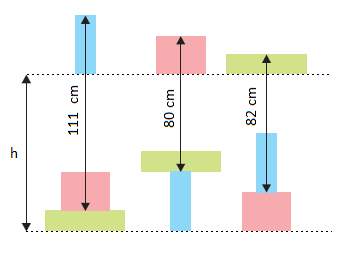
\includegraphics[scale=0.8]{img/fig_05_01.png}}
\end{problem}
\begin{solution}
Sejam $x$, $y$ e $z$ as respectivas alturas dos retângulos azul, vermelho e verde. Na primeira pilha de retângulos, na seta de altura 111 cm, se desconsiderarmos a altura do retângulo azul, obtemos uma seta de tamanho $111-x$. Adicionando o retângulo verde da parte de baixo, obtemos uma seta de altura $111-x+z$ que também tem altura $h$. Ou seja, obtemos a equação $111-x+z=h$. Repetindo esse raciocínio para as outras duas figuras, obtemos equações que formam os seguinte sistema linear.

$$\left\{ \begin{array}{ccc}
111-x+z & = & h  \\
80-y+x  & = & h  \\
82-z+y  & = & h  \end{array}\right.$$

Somando essas três equações obtemos $3h=273$. Daí $h=91$.
\end{solution}

% Exercício 4
\begin{problem}
Na cantina da escola, Alice comprou 5 balas, 2 chicletes, 1 doce e pagou R\$ 6,20;
Bia comprou 6 balas, 2 chicletes, 2 doces e pagou R\$ 9,80;
Cida comprou 8 balas, 3 chicletes e 2 doces. Quanto Cida pagou?
\end{problem}
\begin{solution}
Seja $b$ o valor unitário de uma bala, seja $c$ o valor unitário de um chiclete e seja $d$ o valor unitário de um doce.
Considerando os valores pagos por Alice e por Bia temos que:

$$\left\{\begin{array}{rrrrrrr}
 5b & + &   2c & + &    d & = &   6,20 \\
 6b & + &   2c & + &   2d & = &   9,80
\end{array} \right.$$

Queremos saber o valor da expressão $8b + 3c + 2d$.
Para fazer isso, no sistema anterior, vamos multiplicar a primeira equação por $x$ e vamos multiplicar a segunda equação por $y$, obtendo

$$\left\{\begin{array}{rrrrrrr}
 5xb & + &   2xc & + &    xd & = &   6,20x \\
 6yb & + &   2yc & + &   2yd & = &   9,80y
\end{array} \right.$$

A soma dessas duas equações pode ser colocada na forma

$$(5x+6y)b + (2x+2y)c + (x+2y)d = 6,20x + 9,20y$$

Vamos determinar $x$ e $y$ para os coeficientes de $b$, $c$ e $d$ dessa igualdade serem os mesmos da expressão  $8b + 3c + 2d$ que queremos calcular. Igualando coeficiente a coeficiente, então, vamos determinar $x$ e $y$ de modo que

$$\left\{\begin{array}{rrrrrrr}
 5x & + &  6y & = &   8 \\
 2x & + &  2y & = &   3 \\
  x & + &  2y & = &   2 
\end{array} \right.$$

Resolvendo esse sistema linear com três equações e duas incógnitas obtemos $x=1$ e $y=1/2$. Daí concluímos que

$$8b + 3c + 2d =6,20x + \dfrac{9,80}{2} = 6,20 + 4,90 = 11,10$$

Portanto Cida pagou R\$ 11,10.
\end{solution}

% Exercício 5
\begin{problem}
Paulinho tem peças com cinco formas diferentes (cubos, pirâmides, esferas, cilindros e cones).
Peças com a mesma forma têm o mesmo peso (massa).
Ele coloca algumas peças numa balança de pratos e observa o equilíbrio nas duas situações abaixo.

\centerline{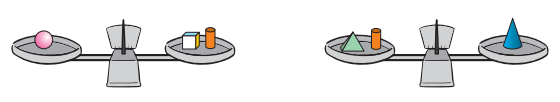
\includegraphics[scale=0.8]{img/fig_05_02.png}}

Com alguns pesos conhecidos, Paulinho observou a situação de equilíbrio abaixo.

\centerline{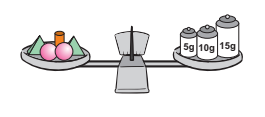
\includegraphics[scale=0.8]{img/fig_05_03.png}}

\begin{enumerate}
\item[(a)] Quanto pesam, juntos, um cubo, uma pirâmide, uma esfera, um cilindro e um cone?
\item[(b)] Quanto pesam, juntos, três cubos, cinco pirâmides, nove esferas, dois cilindros e sete cones?
\end{enumerate}
\end{problem}
\begin{solution}
\begin{enumerate}
\item[(a)] Acrescentando uma pirâmide de cada lado da balança na primeira situação de equilíbrio, vemos que uma esfera mais uma pirâmide pesam o mesmo que um cubo, mais um cilindro, mais uma pirâmide.

\centerline{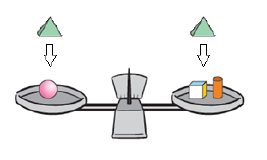
\includegraphics[scale=0.8]{img/fig_05_04.png}}

Da segunda situação de equilíbrio, sabemos que uma pirâmide e um cilindro, juntos, pesam o mesmo que um cone.
Logo, na balança acima, depois de acrescentadas as pirâmides em ambos os pratos, podemos trocar, no segundo prato, a pirâmide e o cilindro por um cone, obtendo a seguinte situação de equilíbrio.

\centerline{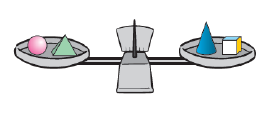
\includegraphics[scale=0.8]{img/fig_05_05.png}}

Agora, olhando para a seguinte situação de equilíbrio 

\centerline{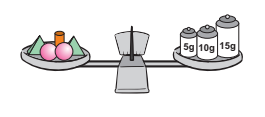
\includegraphics[scale=0.8]{img/fig_05_03.png}}

podemos trocar uma esfera e uma pirâmide por um cone e um cubo, obtendo

\centerline{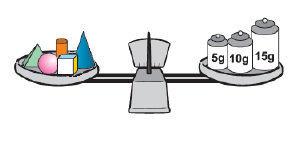
\includegraphics[scale=0.8]{img/fig_05_06.png}}

Assim, os cinco sólidos diferentes, juntos, pesam 30 gramas.

\item[(b)] Poderíamos resolver esse item como o anterior, manipulando as formas geométricas nos pratos, mantendo o equilíbrio da balança. 
Em vez de fazer isso, dessa vez, vamos adotar uma abordagem algébrica da questão.
Vamos, então, representar por $x_1$, $x_2$, $x_3$, $x_4$ e $x_5$ os respectivos pesos de um cubo, de uma pirâmide, de uma esfera, de um cilindro e de um cone.

\centerline{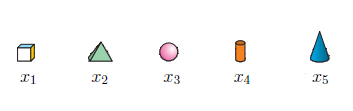
\includegraphics[scale=1]{img/fig_05_07.png}}

As três situações de equilíbrio apresentadas no enunciado podem ser representadas pelas equações

$$x_3 = x_1 + x_4$$
$$x_2 + x_4 = x_5$$
$$2x_2 + 2x_3 + x_4 = 30$$

Essas equações formam um sistema linear com cinco incógnitas e três equações

$$\left\{\begin{array}{rrrrrrrrrrr}
  x_1   &   &           & - &   x_3   & + &    x_4    &   &        & = &    0 \\
        &   &    x_2    &   &         & + &    x_4    & - &   x_5  & = &    0 \\
        &   &   2x_2    & + &  2x_3   & + &    x_4    &   &        & = &    30 \end{array}\right.$$ 

Como desejamos calcular o peso acumulado de três cubos, cinco pirâmides, nove esferas, dois cilindros e sete cones, estamos interessados no valor da expressão

$$3x_1 + 5x_2 + 9x_3 + 2x_4 + 7x_5$$

Para fazer isso, vamos multiplicar a primeira equação do sistema por um número $A$, vamos multiplicar a segunda equação do sistema por um número $B$ e vamos multiplicar a terceira equação do sistema por um número $C$, obtendo

$$\left\{\begin{array}{rrrrrrrrrrr}
  Ax_1   &   &            & - &   Ax_3   & + &    Ax_4    &   &         & = &    0 \\
         &   &    Bx_2    &   &          & + &    Bx_4    & - &   Bx_5  & = &    0 \\
         &   &   2Cx_2    & + &  2Cx_3   & + &    Cx_4    &   &         & = &    30C \end{array}\right.$$ 

Somando essas três equações obtemos a igualdade

$$Ax_1 + (B+2C)x_2 + (-A+2C)x_3 + (A+B+C)x_4 - Bx_5 = 30C$$

Agora vamos calcular os valores de $A$, $B$ e $C$ para os coeficientes de $x_1$ a $x_5$ nessa equação serem iguais aos respectivos coeficientes da desejada expressão $3x_1 + 5x_2 + 9x_3 + 2x_4 + 7x_5$. Igualando coeficiente a coeficiente obtemos as equações

$$\left\{\begin{array}{rrrrrrr}
 A  &   &      &   &           & = &   3 \\
    &   &   B  & + &     2C    & = &   5 \\
-A  &   &      & + &     2C    & = &   9 \\
 A  & + &   B  & + &      C    & = &   2 \\
    &   &  -B  &   &           & = &   7  \end{array}\right.$$

Resolvendo esse sistema linear com cinco equações e três incógnitas obtemos $A=3$, $B=-7$ e $C=6$.
Daí, finalmente, obtemos 

$$3x_1 + 5x_2 + 9x_3 + 2x_4 + 7x_5 = 30C = 180\ kg$$
\end{enumerate}
\end{solution}

% Exercício 6
\begin{problem}
Luciana tem notas de 2 reais, ela tem notas de 5 reais e ela tem notas de 10 reais, totalizando 200 reais.
Ao todo ela possui 34 notas. O que podemos dizer da quantidade de notas que Luciana possui de cada um desses valores?
\end{problem}
\begin{solution}
Se $x$ é a quantidade de notas de 2 reais, se $y$ é a quantidade de notas de 5 reais e se $z$ é a quantidade de notas de 10 reais de Luciana, então as informações da questão podem ser reformuladas no seguinte sistema linear

$$\left\{\begin{array}{rrrrrrr}
  x & + &   y & + &    z & = &   34  \\
 2x & + &  5y & + &  10z & = &  200  \\
\end{array} \right.$$

Efetuando a operação elementar $L_2 \leftarrow L_2 - 2L_1$ obtemos

$$\left\{\begin{array}{rrrrrrr}
  x & + &   y & + &    z & = &   34  \\
    &   &  3y & + &   8z & = &  132  \\
\end{array} \right.$$

Dividindo a segunda linha por 3 obtemos

$$\left\{\begin{array}{rrrrrrr}
  x & + &   y & + &               z & = &   34  \rule{0pt}{15pt} \\
    &   &   y & + &   \dfrac{8}{3}z & = &   44  \rule{0pt}{24pt} \\
\end{array} \right.$$

Efetuando a operação elementar $L_1 \leftarrow L_1 - L_2$ obtemos

$$\left\{\begin{array}{rrrrrrr}
  x &   &     & - &   \dfrac{5}{3}z & = &  -10  \rule{0pt}{15pt} \\
    &   &   y & + &   \dfrac{8}{3}z & = &   44  \rule{0pt}{25pt} \\
\end{array} \right.$$

Observe que este sistema está na forma escalonada reduzida. Considerando $z$ como variável livre, a solução geral do sistema é

$$x = -10 + \dfrac{5}{3}z \ \ \ , \ \ \ y = 44 - \dfrac{8}{3}z \ \ \ , \ \ \ \forall z $$

Agora precisamos voltar para o enunciado e interpretar o significado das variáveis $x$, $y$ e $z$.
Essas variáveis representam as quantidades de notas de 2 reais, de 5 reais e de 10 reais de Luciana.
Logo essas variáveis devem assumir valores que são números inteiros positivos. Para $x>0$ e para $y>0$ obtemos as restrições

$$6 < z < \dfrac{33}{2}=16,5$$

Além disso, como $x$ e $y$ devem ser números inteiros, vemos que $z$ deve ser um  múltiplo de 3. Nesse intervalo, os únicos múltiplos de 3 são $z=9$ ou $z=12$ ou $z=15$. Para cada um desses casos obtemos uma solução possível.

\begin{itemize}
\item $x=5$, $y=20$ e $z=9$.
\item $x=10$, $y=12$ e $z=12$.
\item $x=15$, $y=4$ e $z=15$.
\end{itemize}

Então Luciana pode ter qualquer uma dessas quantidades de notas e isso é o máximo que podemos dizer sobre a quantidade de notas de Luciana de cada um dos valores. O interessante dessa questão é chamar a atenção para, em problemas de aplicação, após obter uma solução algébrica para um sistema linear, voltar e interpretar corretamente a solução e as incógnitas de acordo com o contexto.
\end{solution}

% Exercício 7
\begin{problem}
Quatro irmãos têm conjuntamente quarenta e oito reais. Se, ao dinheiro do primeiro se aumentasse três reais, ao do segundo se retirasse três reais, se o do terceiro triplicasse e o do quarto se reduzisse a um terço, passariam a ter todos a mesma importância. Quanto tem cada um dos quatro irmãos?
\end{problem}
\begin{solution}
Vamos representar por $a$, $b$, $c$ e $d$ as quantias de cada um dos irmão de modo que 
$$a+3 = b-3 = 3c = \dfrac{d}{3}$$
Como a soma das quantias é 48 reais temos que $a+b+c+d=48$ ou, de modo equivalente,
$$(a+3) + (b-3) + c + d =48$$
Substituindo, nessa igualdade, 
$$a+3=\dfrac{d}{3}\ \ \ \ \ \ \ \ b-3=\dfrac{d}{3}\ \ \ \ \ \ \ \ c=\dfrac{d}{9}$$
obtemos
$$\dfrac{d}{3} + \dfrac{d}{3} + \dfrac{d}{9} + d =48 .$$
Multiplicando por 9 obtemos
$$3d + 3d + d + 9d =  432$$
Resolvendo essa equação obtemos $d=27$. Daí segue que
$$a = \dfrac{d}{3}-3 = 9-3=6\ \ \ \ \ \ \ b = \dfrac{d}{3}+3 = 9+3=12 \ \ \ \ \ \ c = \dfrac{d}{9} = 3$$
As quantias dos quatro irmãos são 6, 12, 3 e 27 reais. Observe que:
\begin{itemize}
\item Somando 3 a 6 obtemos 9.
\item Subtraindo 3 de 12 obtemos 9.
\item Multiplicando 3 por 3 obtemos 9.
\item Dividindo 27 por 3 obtemos 9.
\end{itemize}
\end{solution}

% Exercício 8
\begin{problem}
Os amigos Aldo, Beto e Carlos colecionam figurinhas.
Num final de semana eles disputaram três partidas de xadrez.  
Em cada uma dessas três partidas o perdedor teve que dar certa quantidade de figurinhas para os outros dois amigos de modo a dobrar a quantidade de figurinhas do respectivo amigo. 
Na primeira partida Aldo perdeu, na segunda partida Beto perdeu e na terceira partida Carlos perdeu.
No final das três partidas cada um deles ficou com 80 figurinhas.
Quantas figurinhas cada um deles tinha antes de ser disputada a primeira partida de xadrez?
\end{problem}
\begin{solution}
	extbf{Primeira solução.}
Vamos representar por $x$, $y$ e $z$ as quantidades iniciais de figurinhas de Aldo, Beto e Carlos, respectivamente.
\begin{itemize}
\item Quando Aldo perdeu sua partida, ele pagou $y$ para Beto e $z$ para Carlos. Assim eles ficaram, respectivamente, com
$x-y-z$, $2y$ e $2z$ figurinhas.
\item Quando Beto perdeu sua partida, ele pagou $x-y-z$ para Aldo e $2z$ para Carlos. Assim, os três amigos ficaram respectivamente com
$2(x-y-z)$, $2y-(x-y-z)-2z=-x+3y-z$ e $4z$ figurinhas.
\item Quando Carlos perdeu sua partida, ele pagou $2(x-y-z)$ para Aldo e $-x+3y-z$ para Beto. Portanto, no final, eles ficaram respectivamente com $4(x-y-z)$, $2(-x+3y-z)$ e $4z - 2(x-y-z) - (-x+3y-z) = -x-y+7z$ figurinhas.
\end{itemize}
Como eles ficaram com 80 figurinhas cada, podemos montar o seguinte sistema linear.
$$\left\{\begin{array}{rrrrrrr}
4(x-y-z)    & = & 80  \\
2(-x+3y-z)  & = & 80 \\
-x-y+7z     & = & 80 \\ \end{array}\right.$$Simplificando, obtemos
$$\left\{\begin{array}{rrrrrrr}
   x & - &   y  & - &    z & = &   20  \\
  -x & + &  3y  & - &    z & = &   40  \\
	-x & - &   y  & + &   7z & = &   80  \\
\end{array} \right.$$Resolvendo esse sistema linear obtemos como solução $x=130$, $y=70$ e $z=40$. Portanto Aldo, Beto e Carlos tinhas, respectivamente, 130, 70 e 40 figurinhas.
\medskip
	extbf{Segunda solução.}
Essa questão é bem simples e pode ser resolvida sem álgebra alguma. Para isso é suficiente analisar a situação de três para frente.
Sabemos que no final cada um dos três ficou com 80 figurnhas. 
Agora vamos voltar partida a partida e ver quantas figurinhas cada um deles tinha antes dessa partida. 
Voltando uma partida, vamos determinar quantas figurinhas eles tinham antes de Carlos pagar por ter perdido sua partida. Observe que após pagar os dois amigos, as quantidades de figurinhas de Aldo e Beto dobraram.
Logo, cada um deles tinha a metade, 80/2=40 figurinhas. E Carlos tinha as 80 que ficou no final mais o que pagou para os dois amigos.
Logo Carlos tinha 80+40+40=160 figurinhas.
Agora vamos analisar mais um momento anterior. Vamos identificar quanto eles tinham antes de Beto pagar por ter perdido sua partida.
De modo análogo, quando Beto pagou para os dois amigos, as quantidades de figurinhas deles dobraram.
Assim, Aldo tinha 40/2=20 e Carlos tinha 160/2=80. 
Beto tinha, então, as 40 que ficou mais o que pagou, logo Beto tinha 40+20+80=140 figurinhas.
Voltando para o instante inicial, vamos determinar quanto eles tinham antes de Aldo pagar por ter perdido sua partida.
Observe que quando Aldo pagou para os dois amigos por ter perdido sua partida, as quantidades de figurinhas deles dobraram.
Logo Beto tinha 140/2=70 e  Carlos tinha 80/2=40.
E para terminar, temos que Aldo tinha as 20 que ficou mais o que pagou para os amigos, logo Aldo tinha 20+70+40=130 figurinhas.
Portanto, no início, as quantidades iniciais eram Aldo=130, Beto=70 e Carlos=40.
\medskip
Observe que em cada instante, somando os números das linhas da tabela anterior, a soma das quantidades de figurinhas dos três amigos é constante igual a 240.
\end{solution}

% Exercício 9
\begin{problem}
O Gato de Botas, quando vai de sua casa à padaria usando suas botas, demora $20$ minutos, mas quando vai sem suas botas demora $25$ minutos. Se, usando botas, sua velocidade é $6\ Km/h$ a mais do que quando não usa botas, qual a distância de sua casa até a padaria?
\end{problem}
\begin{solution}
Sabemos que a velocidade pode ser escrita como a razão entre uma distância percorrida e o tempo que se levou nesse percurso. Sejam: $x$ a distância entre a padaria e a casa do Gato de Botas, $v$ a velocidade em quilômetros por hora sem as botas e $v+6$ a velocidade em quilômetros por hora com as botas. Do enunciado, quando ele usa as botas, o tempo gasto é 20 minutos, ou seja, é $\dfrac{20}{60}=\dfrac{1}{3}$ de hora. Já quando o gato vai sem as botas, o tempo gasto é de 25 minutos, que corresponde a $\dfrac{25}{60}=\dfrac{5}{12}$ horas.
\begin{itemize}
\item Quando o gato vai sem as botas podemos escrever a velocidade como 
$$v = \dfrac{x}{5/12}$$
\item Quando o gato vai com as botas podemos escrever a velocidade como
$$v+6 = \dfrac{x}{1/3}$$
\end{itemize}
Resolvendo esse sistema de equações obtemos $v=24\ km/h$ e $x=10\ km$.
\end{solution}

% Exercício 10
\begin{problem}
Antigamente existiam marcianos de 3 cores diferentes: vermelhos, verdes e azuis. Como Marte foi devastada por uma guerra intergaláctica, sobraram apenas 2 marcianos de cada uma das cores. Para reconstruir a população marciana, eles decidiram usar uma máquina que transforma dois marcianos, de cores distintas, em quatro marcianos com a cor diferente dos dois iniciais. Por exemplo, se um marciano vermelho e um marciano azul usassem a máquina, eles seriam transformados em quatro marcianos verdes.
\begin{enumerate}
\item[(a)] É possível que, após usar essa máquina um número finito de vezes, tenhamos
2024 marcianos vermelhos, 2024 marcianos verdes e 2024 marcianos azuis?
\item[(b)] É possível que, após usar essa máquina um número finito de vezes, tenhamos
2023 marcianos vermelhos, 2024 marcianos verdes e 2025 marcianos azuis?
\end{enumerate}
\end{problem}
\begin{solution}
\begin{enumerate}
\item[(a)] Existem três tipos de uso da máquina.
\begin{itemize}
\item Tipo 1: quando entra um marciano vermelho e um marciano verde e saem quatro marcianos azuis.
\item Tipo 2: quando entra um marciano vermelho e um marciano azul e saem quatro marcianos verdes.
\item Tipo 3: quanto entra um marciano verde e um marciano azul e saem quatro  marcianos vermelhos.
\end{itemize}
A tabela a seguir ilustra o uso consecutivos desses três tipos da máquina.
\bigskip
\centerline{\begin{tabular}{|c|c|c|c|c|} \hline
         & Vermelho  &  Verde  &  Azul  &  Total  \\  \hline
Início   &    2      &    2    &   2    &    6    \\  \hline
Tipo 1   &    1      &    1    &   6    &    8    \\  \hline
Tipo 2   &    0      &    5    &   5    &   10    \\  \hline
Tipo 3   &    4      &    4    &   4    &   12    \\  \hline
Tipo 1   &    3      &    3    &   8    &   14    \\  \hline
Tipo 2   &    2      &    7    &   7    &   16    \\  \hline
Tipo 2   &    6      &    6    &   6    &   18    \\  \hline  \end{tabular}}
\bigskip
Observe que quando a máquina é utilizada três vezes, cada vez de um tipo, as quantidades de marcianos ficam igual. Logo, repetindo essa sequência, utilizando 1011 vezes cada uma das máquinas, obtemos 2024 marcianos de cada uma das cores.
\item[(b)]  Se o tipo 1 é utilizado $x$ vezes, o tipo 2 é utilizado $y$ vezes e o tipo 3 é utilizado $z$ vezes então a quantidade de marcianos é:
$$vermelho = 2 - x - y + 4z$$
$$verde = 2 - x + 4y - z$$
$$azul = 2 + 4x - y - z$$
Como queremos que essas quantidades sejam, respectivamente, iguais a 2023, 2024 e 2025 obtemos o sistema linear
$$\left\{\begin{array}{rrrrrrrrr}
2 & - &   x & - &   y & + &   4z & = &   2023  \\
2 & - &   x & + &  4y & - &    z & = &   2024  \\
2 & + &  4x & - &   y & - &    z & = &   2025  \end{array}\right.$$
A solução desse sistema linear é
$$x = \dfrac{5056}{5} \ \ \ \ \ \ \ y=1011\ \ \ \ \ \ z=\dfrac{5054}{5}$$
Como $x$ e $z$ não são números inteiros, é impossível que as quantidades de marcianos vermelhos, verdes e azuis sejam respectivamente 2023, 2024 e 2025. Nessa questão também vale a pena chamar a atenção para a necessidade de sempre manter em mente a interpretação dos dados e o significado das incógnitas dentro do contexto que está sendo analisado.
\bigskip\bigskip
Observamos que o item (a) poderia ser resolvido de maneira análoga ao que foi feito no item (b).
Se esse fosse o caso, como devem existir 2024 marcianos de cada cor, obteríamos o seguinte sistema linear.
$$\left\{\begin{array}{rrrrrrrrr}
2 & - &   x & - &   y & + &   4z & = &   2024  \\
2 & - &   x & + &  4y & - &    z & = &   2024  \\
2 & + &  4x & - &   y & - &    z & = &   2024  \end{array}\right.$$
Resolvendo esse sistema, obtemos $x=1011$, $y=1011$ e $z=1011$.
\end{enumerate}
\end{solution}

